%
% 6.857 homework template
%
% NOTE:
% Be sure to define your team members with the \team command
% Be sure to define the problem set with the \ps command
% Be sure to use the \answer command for each of your answers 
\documentclass[11pt]{article}

\newcommand{\team}{ Erica Du \\ Skanda Koppula \\ Jessica Wang }
\newcommand{\ps}{ Problem Set 1 }

%\pagestyle{headings}
\usepackage{amsfonts}
\usepackage{graphicx}
\usepackage{amssymb}
\usepackage{amsmath}
\usepackage{latexsym}
\setlength{\parskip}{1pc}
\setlength{\parindent}{0pt}
\setlength{\topmargin}{-3pc}
\setlength{\textheight}{9.5in}
\setlength{\oddsidemargin}{0pc}
\setlength{\evensidemargin}{0pc}
\setlength{\textwidth}{6.5in}

\newcommand{\answer}[1]{
\newpage
\noindent
\framebox{
	\vbox{
		6.857 Homework \hfill {\bf \ps} \hfill \# #1  \\ 
		\team \hfill \today
	}
}
\bigskip

}


\begin{document}

\answer{1-1 - An edX Security Policy}

\textbf{Objective}: The EdX MOOC platform aims to provide educational content to users of the platform. The platform includes other auxiliary objectives such as being able to update course content, provide inter-person interactivity, and reward users for course completion.\\

\textbf{Principals and Authorized Behavior}: The platform has three main roles: student, teacher, and administrator. Each have their own set of allowed functions:
\begin{itemize}
\item Student: a student must be able to request enrollment into a course, view content for an  enrolled courses (to the extent allowed by course instructor(s)), submit digitally signed answers and feedback to (enrolled) course instructor, modify their own profile information (login username, password, email), and receive certificate of completions as determined by the instructor.
\item Teacher: authorize student enrollment into their course, authorize other instructors to co-administer their course, modify course meta-data (name, description) and content, send signed feedback to student, view the submissions of student enrolled in their course(s), modify their own profile information (email, login username, password), add new course, and award certificate of completion to select student users.
\item Administrator: add teacher user accounts.
\end{itemize}

\textbf{Confidentiality/Integrity Details:}: Specifically, by use of some security mechanism (perhaps, OAuth 2.0 or like), we intend that the platform forbids the student viewing or modify the content and progress of other users (except to view the content of their enrolled courses as allowed by their course instructors). The student should not be able to obtain completion certificates without proper authentication.\\

The teacher should not be able to view the submissions of students not currently in their course. They should not be able to update the content of the courses that they were not authorized to administer.


\answer{1-2 - Reused Pad Cipher}
A. Suppose we apply the XOR function on two bits A and B: XOR(A,B)=C. Given B and C, we can determine A (specifically, XOR(B,C)=A). We can show this by enumerating all four possibilities in the XOR input table: \\
\begin{center}
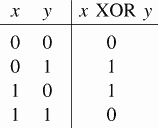
\includegraphics{xor-table.png}
\end{center}

That means that given a byte of ciphertext, there are twenty-six possibilities for the corresponding byte in the pad (we know all bytes in the plain text are alphabetic characters). We can choose among these 26 possibilities by seeing which pad XOR'd with the corresponding byte in the other ciphertext produces a alphabetic character. If none of the 26 possibilities result in the other ciphertext decrypting to an alphabetic character, we can assume the two ciphertexts came from two different pads. If more than one possibility produces an alphabetic character, we can determine which one by moving on to the next byte, applying the same analysis and examining at the end which one produces a dictionary word.

The following Python script does this for us:

B. 


\answer{1-3 - Vulnerability/Mechanism Chains}



\end{document}

